\documentclass[border=3pt,tikz]{standalone}
\usepackage{amsmath}
\usetikzlibrary{arrows.meta}
\usetikzlibrary{calc}
\begin{document}
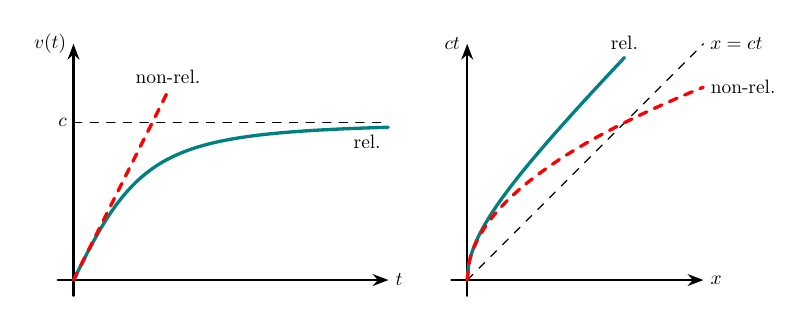
\begin{tikzpicture}[line cap=round, scale = 2]

    \draw [thick, -{Stealth[length=2mm]}] (-0.1, 0) -- (2, 0) node [right, scale=0.7] {$t$};
    \draw [thick, -{Stealth[length=2mm]}] (0, -0.1) -- (0, 1.5) node [left, scale=0.7] {$v(t)$};
    
    
    \def\a{2.0};
    \def\b{1.0};
    \draw[dashed] (0, 1) -- (2, 1);
    \draw[very thick, teal] plot[variable=\t,domain=0:2, samples=100, smooth,thick] ({\t}, {\a*\t/sqrt(1+(\a*\t)^2)}) node[below left, scale=0.7, black] {rel.};
    \draw[very thick, dashed, red] (0, 0) -- (0.6, 1.2) node[above, scale=0.7, black] {non-rel.};
    \node [left, scale=0.7] at (0, 1) {$c$}; 
    
    
    \begin{scope}[shift={(2.5,0)}]
    \draw [thick, -{Stealth[length=2mm]}] (-0.1, 0) -- (1.5, 0) node [right, scale=0.7] {$x$};
    \draw [thick, -{Stealth[length=2mm]}] (0, -0.1) -- (0, 1.5) node [left, scale=0.7] {$ct$};
    
    \draw [dashed] (0, 0) -- (1.5, 1.5) node[right, scale=0.7] {$x=ct$};
    
    \draw[very thick, teal] plot[variable=\t,domain=0:1.0, samples=100, smooth,thick] ({\t}, {sqrt((\t+1/\a)^2 -1/(\a^2))}) node [above, scale=0.7, black] {rel.};
    \draw[very thick, dashed, red] plot[variable=\t,domain=0.0:1.5, samples=100, smooth,thick] ({\t}, {sqrt(2*\t/\a)}) node [right, scale=0.7, black] {non-rel.};
    
    \end{scope}
    \end{tikzpicture}
\end{document}